\section{抽象语法树AST}
AST是MiniC采用的第一重中间表示,它由在词法/语法分析阶段生成。由于我们在AST上完成了符号表的生成和类型检查,因此这两部分也在本章介绍。
\subsection{生成}
AST的结构是根据上下文无关文法的产生式定义的:一个终结符节点是一棵AST;一棵以产生式左部非终结符为根的AST的子节点按从左到右顺序分别是其右部分法符号所产生的AST。

比如有如下产生式:
\begin{displaymath}
	A:=aBcD
\end{displaymath}
其中大写字母代表非终结符,小写字母代表终结符,那么以非终结符A为根的AST就是如下形式:
\dirtree{%
.1 A.
.2 a.
.2 以非终结符B为根的AST.
.2 c.
.2 以非终结符D为根的AST.
}
注意到AST的定义实际上也给出了其产生方法:只要在做LR分析时,随着规约的进行,将子树与根进行连接即可。

在实现时,AST的叶节点在词法分析时生成,内部节点在语法分析时在不同的产生式的语法规则指导下生成,并在规约时连接到其父节点上。

下面给出一个MiniC的AST节点所包含的内容:
\begin{lstlisting}
typedef struct AST_NODE{
  	int nodeType;//节点类型,即节点代表了哪个文法符号
  	int nodeLevel;//节点深度
	union node_content content; //节点包含的内容,只有叶子节点才不为空,在词法分析时添加
  	AST_NODE * father;//父节点
  	AST_NODE * leftChild;//最左子节点
  	AST_NODE * rightSibling;//右兄弟节点

	struct symtbl_hdr* symtbl;//文法符号所在范围的符号表
	AST_NODE* double_list;
}AST_NODE;
\end{lstlisting}
{\it \anchor 有关节点类型的详细定义,请参阅:\verb|AST.h|}\\
{\it \anchor 有关建立AST树的相应过程,请参阅:\verb|AST_operation.c|, \verb|minic.y|}\\
\subsection{生成的语法树示例}
我们利用\verb|dot|生成了下面代码的AST:
\begin{lstlisting}
int main()
{
	int i;
	i = i + 1;
}

\end{lstlisting}

\begin{center}
	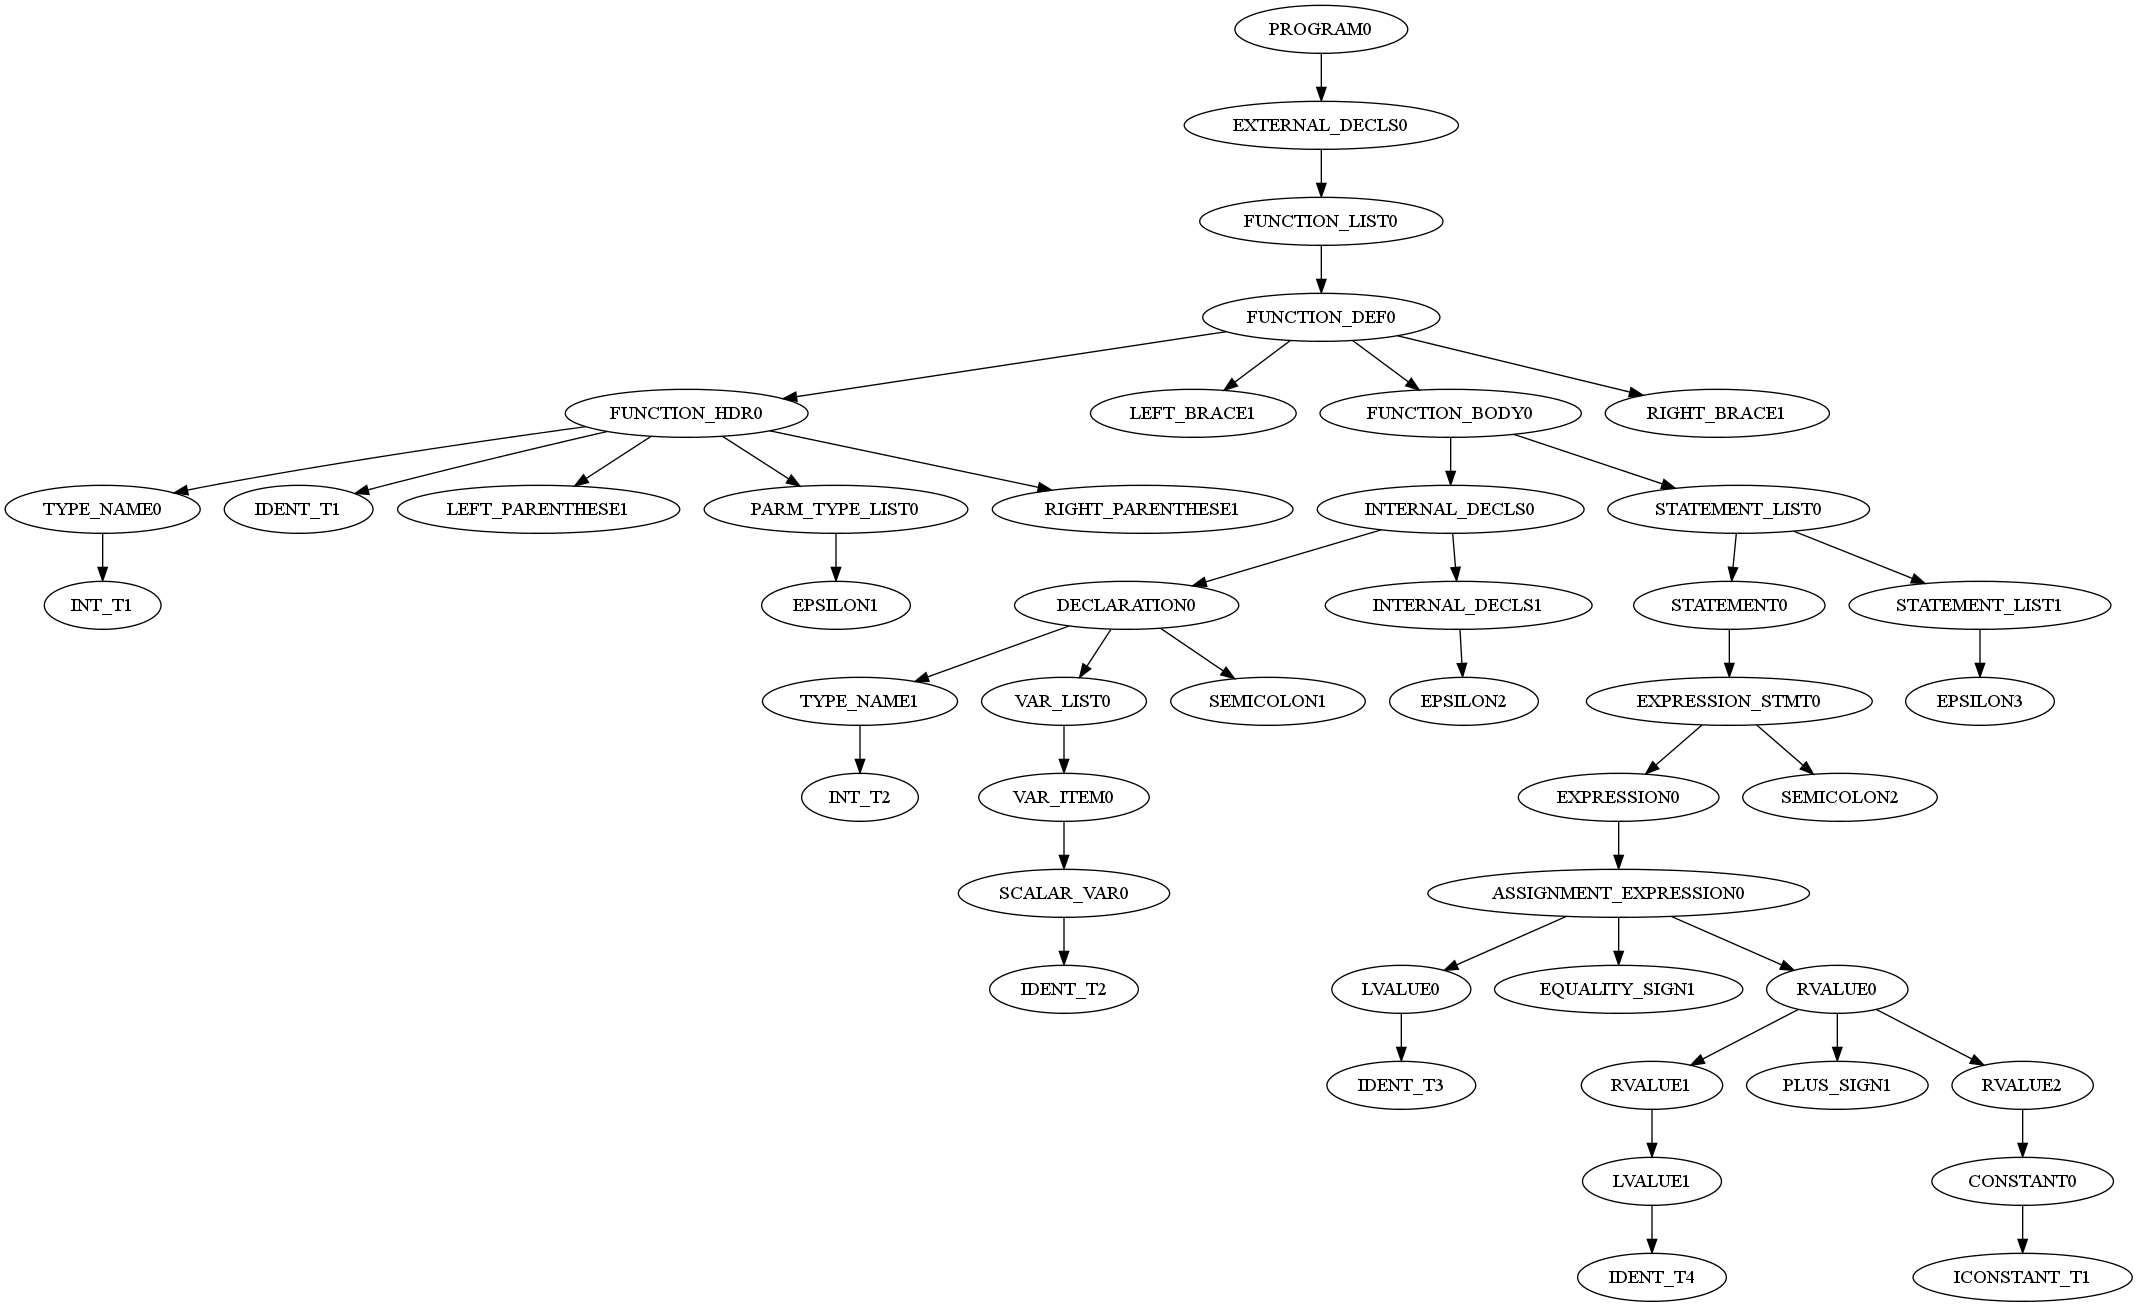
\includegraphics[scale=0.2]{grammer_tree.png}
	\captionof{figure}{AST示例}
	\label{fig:grammertree}
\end{center}
{\it \manerrarrow MiniC的验证工具中提供了两种方式查看输入源文件的语法树:\verb|dot|和ASCII ART,请参阅MiniC使用手册}\\
\subsection{符号表}
符号表对于一个编译程序而言是最为重要的一个部分,从它创建以后开始的每一个步骤中,“标识符”(函数名、变量名)的出现,就意味着要在符号表中找到对应的表项,提取要使用的信息。

\paragraph*{符号表的结构}
符号表的层次结构需要根据语言的特性来决定。例如在MiniC中,由于存在着全局变量、函数声明、语句块等特点,因此符号表需要组织成树状结构。

符号表的具体底层数据结构可以有很多种选择,常见的有哈希表、链表和线性表,在MiniC中,由于考虑到输入源文件的规模都较小,所以采用可扩张的线性表来实现\footnote{这种线性表在空间不足时会另外申请一块两倍的空间并拷贝自己}。在这种实现下,插入一个表项的均摊开销是$O(1)$,检索一个表项的开销是$O(n)$,$n$为表项总数目。


MiniC的符号表结构如下:
\begin{enumerate}
\item 每个作用域(函数、复合语句)一张符号表:
\begin{lstlisting}
struct symtbl_hdr
{
	symtbl_hdr* parent_tbl; //父表
	symtbl_hdr* leftChild_tbl; //最左子表
	symtbl_hdr* rightSibling_tbl;	//右兄弟子表

	//ret_type, ret_star, para_num, func are useful only for function's symtbl
	char* func_name; //函数名,若该表属于复合语句则该项为空
	int ret_type; //函数返回值基类型
	int ret_star; //函数返回值是否为指针类型
	int para_num; //该函数的参数个数
	int func_def; //该函数是否有定义
	int item_num; //符号表表项数目
	int maxSize; //全部表项占用的内存大小,字节
	symtbl_item* item; //表项列表
}
\end{lstlisting}
\item 每张符号表都有一个表项列表:
\begin{lstlisting}
struct symtbl_item
{
	int isGlobal; //是否为全局变量
	int type; //表项的基类型
	int star_num; //表项是否为指针
	int writable; //表项是否为只读类型
	char* name; //符号名 
	int size; //数组大小,非数组为0
	int func_off; //
	int offset; //在内存分配中的偏移
};

\end{lstlisting}
\end{enumerate}
注意到在一个函数的符号表中,函数的参数和它的局部变量是存放在一起的,这种将参数和局部变量视作同类的安排能够为以后的内存分配、寄存器分配等提供一些方便。



\paragraph*{在AST上生成符号表}
如前所述,AST上包含了源文件中所有的信息,因此只需要扫描AST的某些子树,提取符号名称、类型、作用域等信息,就可以生成符号表。

具体的做法是:先序深度优先周游AST,找到作用域入口(\verb|FUNCTION_DEF|和\verb|COMPOUND_STMT|)并将当前作用于压入作用域栈,然后在该作用域节点下寻找类型为\verb|EXTERNAL_DECLS|和\verb|INTERNAL_DECLS|的节点,分情况处理该节点的函数和变量的声明,将名称和类型(包括函数的返回类型,参数、参数类型)加入符号表,作用域从作用域栈顶取得。在作用域出口(周游函数返回时)弹出作用域栈顶。\\
{\it \anchor 有关符号表生成的相关代码,请参阅:\verb|gen_symtbl.h|}\\

\paragraph*{在符号表上查询符号}
由于符号表是树状组织,因此查询时要从给定的一张符号表开始,在表中查找,如果未找到符号,就在当前表的父表中查找,直到找到该符号或者在最高级的\verb|Global Scope|也没有找到返回空。
\\
{\it \anchor 有关符号表查询的代码,请参阅:\verb|symtbl_operation.h|}\\
\paragraph*{符号表生成与语义检查}
在符号表生成的过程中,实际上还要进行一项语义检查:同一作用域的多重定义问题。即在向当前符号表中添加符号时,如果该符号已经出现在了当前表中,就要报告错误,停止建立符号表。

\subsection{符号表示例}
下图展示了以下代码的符号表:
\begin{lstlisting}
int i,j;
void f(int k)
{
	int i,j;
}
int main()
{
	int i,j;
	{
		int k;
	}
}
\end{lstlisting}
\begin{center}
	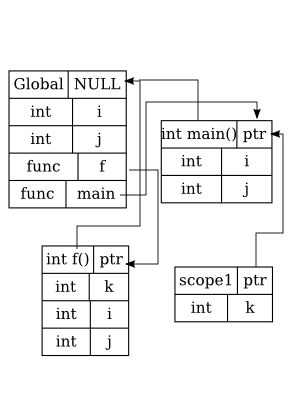
\includegraphics[scale=0.6]{symtbl.png}
	\captionof{figure}{符号表示例}
	\label{symtbl}
\end{center}
{\it \manerrarrow MiniC的验证工具中提供了查看源文件生成的符号表的方法:请参阅MiniC使用手册}\\
\subsection{类型检查}
